\documentclass[
12pt,
a4paper,
bibliography=totocnumbered, %Literaturverzereichnis als Eintrag ins Inhaltsverzeichnis
%twoside, %Zweiseitiger Druck
BCOR=1cm, %Platz zum Lochen
oneside, %Einseitiger Druck
]{scrartcl}

\usepackage{geometry}

\usepackage[default]{fontsetup}
%\usepackage[onehalfspacing]{setspace}

\usepackage[ngerman]{babel}
\usepackage[babel=true,german=quotes]{csquotes}

\usepackage{microtype}
\usepackage{mleftright}
%\newcommand{\Le}{\mleft}
%\newcommand{\Ri}{\mright}
\usepackage[no-script, no-scriptscript, no-inner, no-close]{innerscript}

% Mathepakete (unicode-math ersetzt amssymb, amsfonts etc.)
\usepackage{amsmath,amsthm}
\usepackage{mathtools}
\usepackage{fixdif,derivative}
\usepackage{physics2}
\usephysicsmodule{ab.legacy}

\usepackage{unicode-math}
\setmathfont{NewCMMath-Book}
\setmathfont{NewCMMath-Book}[range=cal, StylisticSet=1]
\setmathfont{NewCMMath-Book}[range=scr]

\usepackage{siunitx}
\sisetup{detect-weight=true, detect-family=true,locale=DE,range-phrase={\,bis\,},list-final-separator ={\,\linebreak[0] \text{und}\,},separate-uncertainty=true,per-mode = symbol-or-fraction}
%\SI[per-mode = fraction]{1}{\meter\per\second} erzwingt auch im Fließtext die Bruchdarstellung.
\DeclareSIUnit\curie{Ci}%Zusätzliche Einheit definieren

\usepackage{tabularx, booktabs, multirow}
\usepackage{array}
\usepackage{enumitem}
\usepackage{float}
\usepackage{graphicx}
\usepackage{xurl}

\usepackage[final]{pdfpages}
\usepackage{framed, color} %Framed: Paket, mittels dessen ein Rahmen um einen Bereich definiert werden kann. Color: Lässt Farbdarstellung in Schrift, Hintergrund etc. zu

\usepackage{scrlayer-scrpage} %Header für die KOMA-script-Klasse

%\usepackage[square,numbers]{natbib}
\usepackage{subfigure} %Mehrere Bilder in einer Figure-Umgebung

\usepackage[bookmarks,colorlinks=true]{hyperref}
\hypersetup{
	colorlinks,
	linktocpage,
	citecolor=black,
	filecolor=black,
	linkcolor=black,
	urlcolor=black,
	pdftitle=X,
	pdfauthor=JM-VS
}

\usepackage[backend=biber, style=chem-angew]{biblatex}
\addbibresource{lit.bib}

\numberwithin{equation}{section} % Die Nummerierung von Gleichungen bekommt die jeweilige Section-Nummer als Präfix

\setlength{\parindent}{0pt} %Einrücktiefe von neuen Absätzen
\setlength{\parskip}{6pt} %Abstand von Absätzen

\pagestyle{scrheadings}%Kopf und Fußzeilen
\ohead{\textbf{\GRUPPENNR\ - \VERSUCHSNR}} %Header oben links auf linker Seite (ungerade Seitenzahl) und oben rechts auf rechter Seite (gerade Seitenzahl), beinhaltet gruppennummer und Versuchskürzel. Im Fall eine einseitigen Dokuments: Header oben rechts
\ihead{\VerfasserEINS\;\&\;\VerfasserZWEI} %Header oben rechts auf linker Seite und oben links auf rechter Seite. Beinhaltet die Namen der Verfasser. Im Fall eine einseitigen Dokuments: Header oben links!
\ofoot{\thepage} %Footer unten links auf linker und unten rechts auf rechter Seite, enthält die jeweilige Seitenzahl. Im Fall eines einseitigen Elements: Footer unten rechts!
\cfoot{\empty} %Mittig unten im Footer soll nichts eingetragen werden
\ifoot{\empty} %Footer unten rechts auf linker und unten links auf rechter Seite. Hier ebenfalls leer.

\newcommand{\tz}{T_{\text{II}}}
\newcommand{\ts}{T_{\text{S}}}
\newcommand{\tgl}{T_{\text{gl}}}
\newcommand{\tgeg}{T_{\text{geg}}}
\newcommand{\omz}{\omega_{\text{II}}}
\newcommand{\omgl}{\omega_{\text{gl}}}
\newcommand{\omgeg}{\omega_{\text{geg}}}
\newcommand{\kB}{k_{\text{B}}}
%%%%%%%%%%%%%%%%%%%%%%%%%%%%%%
% GENERAL

\newcommand{\e}{\mathrm{e}} % Der hier von \eul redefined
\newcommand{\imag}{\mathrm{i}}
%\newcommand{\dif}[1]{\mathrm{d}#1} not needed (fixdif package)
\newcommand{\Le}{\mleft}
\newcommand{\Ri}{\mright}
\newcommand{\RR}{\mathbb{R}}
\newcommand{\ensp}{\enspace}
\newcommand{\sbst}{\subset}
\newcommand{\id}{\mathbb{1}}
\renewcommand{\implies}{\Rightarrow}
\newcommand{\openint}[2]{{]{#1,#2}[}}
\newcommand{\diag}[1]{\mathrm{diag}\Le\{#1\Ri\}}
\DeclarePairedDelimiterXPP\Exp[1]{\operatorname{exp}}{(}{)}{}{#1} %exp Operator mit passendem Klammern Spacing oder so
\newcommand{\bv}[1]{\symbfit{#1}} % bolt vector

%%%%%%%%%%%%%%%%%%%%%%%%%%%%%%
% SYMBOLS

\newcommand{\veps}{\varepsilon}
\newcommand{\vphi}{\varphi}

%%%%%%%%%%%%%%%%%%%%%%%%%%%%%%
% TOPOLGY

\DeclareMathOperator{\accumulated}{acc}
\DeclareMathOperator{\isolated}{iso}
\DeclareMathOperator{\interior}{int}
\DeclareMathOperator{\exterior}{ext}
\newcommand{\edge}{\partial}
\DeclareMathOperator{\CauchySeq}{\text{CF}}

%%%%%%%%%%%%%%%%%%%%%%%%%%%%%%
% LINEAR ALGEBRA

\DeclareMathOperator{\trace}{Tr}
\DeclareMathOperator*{\Vektor}{\scalerel*{V}{\sum}}
\DeclareMathOperator{\core}{ker}
%\DeclareMathOperator{\span}{span}

%%%%%%%%%%%%%%%%%%%%%%%%%%%%%%
% VECTOR CALCULUS

\newcommand{\nbl}{\symbfup{\nabla}}
\DeclareMathOperator{\grad}{grad}
\DeclareMathOperator{\divgc}{div}
\DeclareMathOperator{\rot}{rot}

%%%%%%%%%%%%%%%%%%%%%%%%%%%%%%
% PHYSICS
\newcommand{\poiss}[2]{\Le\{#1,#2\Ri\}} % Poissant brackets

%\prime
%\dprime
%\trprime

% Hier können die individuellen Anpassungen vorgenommen werden, die sich auf das Titelblatt und die Kopfzeilen auswirken.

\newcommand{\VERSUCHSDATUM}{01.10.2025}
\newcommand{\PROTOKOLLDATUM}{\today}

\newcommand{\VerfasserEINS}{Julian Molt}
\newcommand{\MatNoEINS}{3803097}
\newcommand{\StudiengangEINS}{Physik}

\newcommand{\VerfasserZWEI}{Valentin Stopper}
\newcommand{\MatNoZWEI}{3774391}
\newcommand{\StudiengangZWEI}{Physik}

\newcommand{\BETREUER}{Simon Krinke}
\newcommand{\GRUPPENNR}{A-016}

\newcommand{\VERSUCHSNR}{M30}
\newcommand{\VERSUCHSNAME}{Erzwungene Schwingung und Resonanz}


\begin{document}

\thispagestyle{empty}

\begin{titlepage}

	\begin{center}
		\Huge{\textbf{\VERSUCHSNR\ -- \VERSUCHSNAME}}\\
		\vspace{10mm}
		\Large{Protokoll zum Versuch des Physikalischen Praktikums I von \\ \textbf{\VerfasserEINS\;\& \VerfasserZWEI}}\\
		\vspace{10mm}
		\Large{Universität Stuttgart}\\
	\end{center}
	\vspace{1cm}
	\begin{center}
		\begin{tabular}{ll}
			\large{Verfasser:}		& \large{\VerfasserEINS\;(\StudiengangEINS),} \\
			& \large{\MatNoEINS} \\
			\vspace{0cm}\\
			& \large{\VerfasserZWEI\;(\StudiengangZWEI),} \\
			& \large{\MatNoZWEI} \\
			\vspace{0cm}\\
			\large{Gruppennummer:}	& \large{\GRUPPENNR} \\
			\vspace{0cm}\\
			\large{Versuchsdatum:}	& \large{\VERSUCHSDATUM} \\
			\vspace{0cm}\\
			\large{Betreuerin:}		& \large{\BETREUER}
		\end{tabular}
	\end{center}
	\vspace{15mm}

	\begin{center}
		Stuttgart, den \PROTOKOLLDATUM
	\end{center}

\end{titlepage}

\thispagestyle{empty}

\tableofcontents

\clearpage %Neue Seite, davor werden alle noch ausstehenden Grafiken/Tabellen platziert.

\renewcommand{\thepage}{\arabic{page}}
\setcounter{page}{1}

% Die erste eckige Klammer ist optional, die darin angegebene Bezeichnung steht im Inhaltsverzeichnis anstelle des hinteren (längeren) Namens.
\section[Versuchsziel]{Versuchsziel und Versuchsmethode}

Im Versuch wurde die Bewegung eines Drehpendels bei unterschiedlichen Anregungsfrequenzen und Dämpfungen betrachtet. Dazu wurden die Kreisfrequenzen \(\omega_0\) bei verschiedenen Auslenkungen bestimmt. Außerdem wurden das logarithmische Dekrement und die Abklingkonstante \(\delta\) für die gedämpften Schwingungen bestimmt. Zuletzt wurde die Resonanzkurve für die Auslenkung \(\Psi\) der angeregten Schwingungen ermittelt.

\section{Grundlagen}

Beim Auslenken eines Systems aus dem Zustand mit der geringsten potentiellen Energie entstehen rückwirkende Kräfte, durch die eine Schwingung entsteht. Bei Drehpendeln treten die rückwirkenden Kräfte in Form von Drehmomenten auf. Ohne Dämpfung und Anregung erzeugt nur die Spiralfeder mit der Federkonstante $D$ ein Drehmoment, wodurch sich die Differentialgleichung zur Beschreibung des Auslenkwinkels \(\Psi(t)\) mit dem Trägheitsmoment \(J\) ergibt:
\begin{equation}
	J \cdot \odv[2]{\Psi(t)}{t} = 0 \,.
\end{equation}
Die Formel \(\Psi(t) = \alpha \e^{\imag \omega_0 t} + \beta \e^{- \imag \omega_0 t}\) ist die Lösung dieser Differentialgleichung, wobei sich \(\alpha\) und \(\beta\) aus den Anfangsbedingungen ergeben. \(\omega_0\) ist die Eigenfrequenz des System und kann mit
\begin{equation}
	\omega_0 = \sqrt{\frac{D}{J}}
\end{equation}
berechnet werden. Da das rückstellende Drehmoment hier proportional zur Auslenkung ist, handelt es sich um eine harmonische Schwingung.

Bei der gedämpften Schwingung kommt noch ein der Bewegung entgegenwirkendes Drehmoment hinzu. Dieses wirkt nicht proportional zur Auslenkung und sorgt dafür, dass die Amplitude abnimmt. Die Differentialgleichung der gedämpften Schwingung lautet dann
\begin{equation}
	J \cdot \odv[2]{\Psi(t)}{t} + B \cdot \odv{\Psi(t)}{t} + D \cdot \Psi(t) = 0 \,,
\end{equation}
mit der allgemeinen Lösung
\begin{equation}
	\Psi(t) = \e^{\frac{-B}{2J} \cdot t} \cdot \Le[\alpha \e^{\sqrt{\frac{B^2}{4J^2} - \frac{D}{J}}\cdot t} + \beta \e^{-\sqrt{\frac{B^2}{4J^2} - \frac{D}{J}}\cdot t}\Ri] \,.
\end{equation}
Die reelle Eigenfrequenz des Systems ist
\begin{equation}
	\omega_1=\frac{2 \pi}{T_1}=\sqrt{\frac{D}{J}-\frac{B^2}{4J^2}} \,.
\end{equation}
Zur Beschreibung der Dämpfungsstärke wird die Abklingkonstante $\delta$ verwendet. Die Bestimmung dieser kann durch das Verhältnis zweier aufeinanderfolgender Maxima geschehen
\begin{equation}
	\frac{\Psi_n}{\Psi_{n+1}}=e^{\delta T_1} \,.
\end{equation}
Das logarithmische Dekrement \(\Lambda\) ergibt sich, durch die Anwendung des natürlichen Logarithmus
\begin{equation}
	\ln\Le(\frac{\Psi_n}{\Psi_{n+1}}\Ri) = \delta T_1
\end{equation}

Kommt nun eine Anregung, in Form einer externen periodischen Kraft auf das System, hinzu, ergibt sich eine inhomogene Differentialgleichung
\begin{equation}
	J \cdot \odv[2]{\Psi}{t} + B \cdot \odv{\Psi(t)}{t} + D\Psi(t)=M_0\cos(\omega t) \,,
\end{equation}
mit dem äußeren Drehmoment \(M = M_0 \cos(\omega t)\) als Störterm. Die partikuläre Lösung ist, mit Hilfe der Beziehung \(\omega^2_0 = \frac{D}{J}\)
\begin{equation}
	\Psi(t) = \frac{M_0}{\sqrt{J^2(\omega^2_0 - \omega^2)^2 + B^2\omega^2}}\cos(\omega t - \phi) \,.
\end{equation}
Die Phasenverschiebung \(\phi\) kann durch
\begin{equation}
	\tan\phi=\frac{B\omega}{J\Le(\omega^2_0 - \omega^2\Ri)}
\end{equation}
bestimmt werden.

\section[Messprinzip]{Messprinzip mit Abbild und Versuchsablauf}

Abbildung 1 skizziert den Versuchsaufbau. Am schwingenden System (3) wird durch die Spiralfeder (4) ein rückstellendes Drehmoment verursacht. Die Auslenkung aus der Ruhelage und die Amplitude der Schwingung, können über den Zeiger (6) und die Skala (2) bestimmt werden. Gedämpft wird die Schwingung durch den Elektromagnet (1). Die Stromstärke am Elektromagnet, wird über das Multimeter abgelesen (in Abbildung 2 rechts), um die Stärke der Dämpfung abzuschätzen. In Abbildung 2 ist rechts neben dem Schwingungssystem eine kleine Box, diese enthält den Motor zur Erzeugung der externen periodischen Kraft. Diese wird durch das Antriebsrat (11) und die Schubstange (12) zum Drehpendel übertragen. Die äußere Frequenz der Anregenden Kraft kann über die Drehzahlregler (7) eingestellte werden. Zentriert vor dem Drehpendel befindet sich eine Kamera, zur Aufzeichnung der Schwingung.

Die Eigenfrequenz des ungedämpften Systems wurde bestimmt indem, bei ausgeschaltetem Elektromagneten, das Pendel um weniger als 90° ausgelenkt und die Schwingungsdauer über 10 Perioden gestoppt wurde. Das wurde für 5 verschiedene Auslenkungen wiederholt.
Für die Gedämpfte Schwingung wurde dieses Vorgehen wiederholt, allerdings erst mit 0,2 Ampere und dann mit 0,4 Ampere am Elektromagneten, sowie jeweils fünf Auslenkungen über \qty{90}{\degree}.

Für die Bestimmung der Abklingkonstante und des logarithmischen Dekrements wird die Schwingung bei beiden Dämpfungen mit der Kamera aufgezeichnet und mit dem Programm VianaNET ausgewertet. Im Programm wird zunächst die Video Aufnahme gestartet und anschließend die Analyse geöffnet. Dort wird Skalierung und ein Koordinatenursprung gewählt. Anschließend wird für das Bewegungstracking die Farbe des Zeigers makiert. Zuletzt wird die Automatische Analyse gestartet, welche als Ergebnis eine Tabelle und zugehörige Diagramme mit den Bewegungsdaten des Pendels ausgibt. Dadurch ist die Auslenkung über die Zeit und somit das logarithmische Dekrement des Drehpendels bekannt.

Der letzte Versuchsteil ist die Bestimmung der Resonanzkurve. Hier werden für die beiden Dämpfungen jeweils 5 Schwingungen mit Frequenzen über und unter der Eigenfrequenz des Systems, angeregt. Dabei muss bei jeder Frequenz gewartet werden, bis das Pendel eingeschwungen ist. Das bedeutet in der Praxis, dass sich die Amplitude nur noch minimal ändert. Dann kann die Amplitude über die Skala abgelesen und notiert werden.

%\begin{figure}[H]
%	\centering{\includegraphics[width=0.9\textwidth]{X.jpg}}
%	\caption{X.}
%	\label{fig:X}
%\end{figure}

\section{Messwerte}

\begin{table}[H]
	\centering
	\caption{Gemessene Periodendauern \(\Delta T^{10}\) der ungedämpften Schwingung. \label{tbl:ungedämpft}}
	\begin{tabular}{lr}
		\toprule
		Auslenkung in Skalenteilen & \(\Delta T^{10}\) in \si{\second}\\
		\midrule
		11 & \num{19,03}\\
		10 & \num{19,22}\\
		7  & \num{18,87}\\
		\bottomrule
	\end{tabular}
\end{table}

\begin{table}[H]
	\centering
	\caption{Gemessene Periodendauern \(\Delta T^{10}\) der mit \(I = \qty{0,4}{\ampere}\) gedämpften Schwingung. \label{tbl:gedämpft400mA}}
	\begin{tabular}{lr}
		\toprule
		Auslenkung in Skalenteilen & \(\Delta T^{10}\) in \si{\second}\\
		\midrule
		19 & \num{19,06}\\
		17 & \num{19,09}\\
		15 & \num{18,97}\\
		\bottomrule
	\end{tabular}
\end{table}

\begin{table}[H]
	\centering
	\caption{Gemessene Periodendauern \(\Delta T^{10}\) der mit \(I = \qty{0,2}{\ampere}\) gedämpften Schwingung. \label{tbl:gedämpft200mA}}
	\begin{tabular}{lr}
		\toprule
		Auslenkung in Skalenteilen & \(\Delta T^{10}\) in \si{\second}\\
		\midrule
		19 & \num{18,87}\\
		17 & \num{18,97}\\
		15 & \num{19,03}\\
		\bottomrule
	\end{tabular}
\end{table}

\begin{table}[H]
	\centering
	\caption{Amplituden \(\Psi\) der mit \(I = \qty{0,4}{\ampere}\) gedämpften Schwingung, sowie unter Erregerfrequenz \(f\). \label{tbl:MAXgedämpft400mA}}
	\begin{tabular}{lr}
		\toprule
		\(f\) in \si{\hertz} & \(\Psi\) in Skalenteilen\\
		\midrule
		\num{0,41} & \num{1,4}\\
		\num{0,43} & \num{1,6}\\
		\num{0,45} & \num{1,9}\\
		\num{0,51} & \num{4,1}\\
		\num{0,52} & \num{5,1}\\
		\num{0,55} & \num{4,5}\\
		\num{0,58} & \num{2,3}\\
		\bottomrule
	\end{tabular}
\end{table}

\section{Auswertung}

Die Eigenfrequenz \(\omega_0\) kann einfach bestimmt werden durch
\begin{equation*}
	\omega_0 = \frac{2\pi}{\overbar{T}} \,,
\end{equation*}
wobei \(\overbar{T}\) die mittlere Periodendauer \(\overbar{T} = \frac{1}{n} \sum_{i=1}^{n} \frac{\Delta T^{10}_i}{10}\) ist. Hierbei gilt \(n = 3\), weshalb sich die Eigenfrequenz auf
\begin{align*}
	\omega_0 &= \frac{60 \pi}{\Delta T_1^{10} + T_2^{10} + T_3^{10}}\\
			 &= \frac{60\pi}{\Le(\num{19,03} + \num{19,22} + \num{18,87}\Ri)\si{\second}} = \qty{3,30}{\per\second}\,.
\end{align*}

Analog folgen für die Dämpfung mit \(I = \qty{0,4}{\ampere}\) \(\omega_{0,\text{stark}} = \qty{3,30}{\per\second}\) und für die Dämpfung mit \(I =\qty{0,2}{\ampere}\)\(\omega_{0,\text{schwach}} = \qty{3,31}{\per\second}\)

\section{Zusammenfassung}


%\begin{thebibliography}{999}
%	\bibitem{Quelle} Versuchsanleitung zu \emph{E24 -- Halbleiterdioden} (Abgerufen am 29.09.2025).
%	Online verfügbar unter: \url{https://www3.physik.uni-stuttgart.de/studium/praktika/ap/pdf_dateien/E24.pdf}
%\end{thebibliography}

\printbibliography

\section{Anhang}

%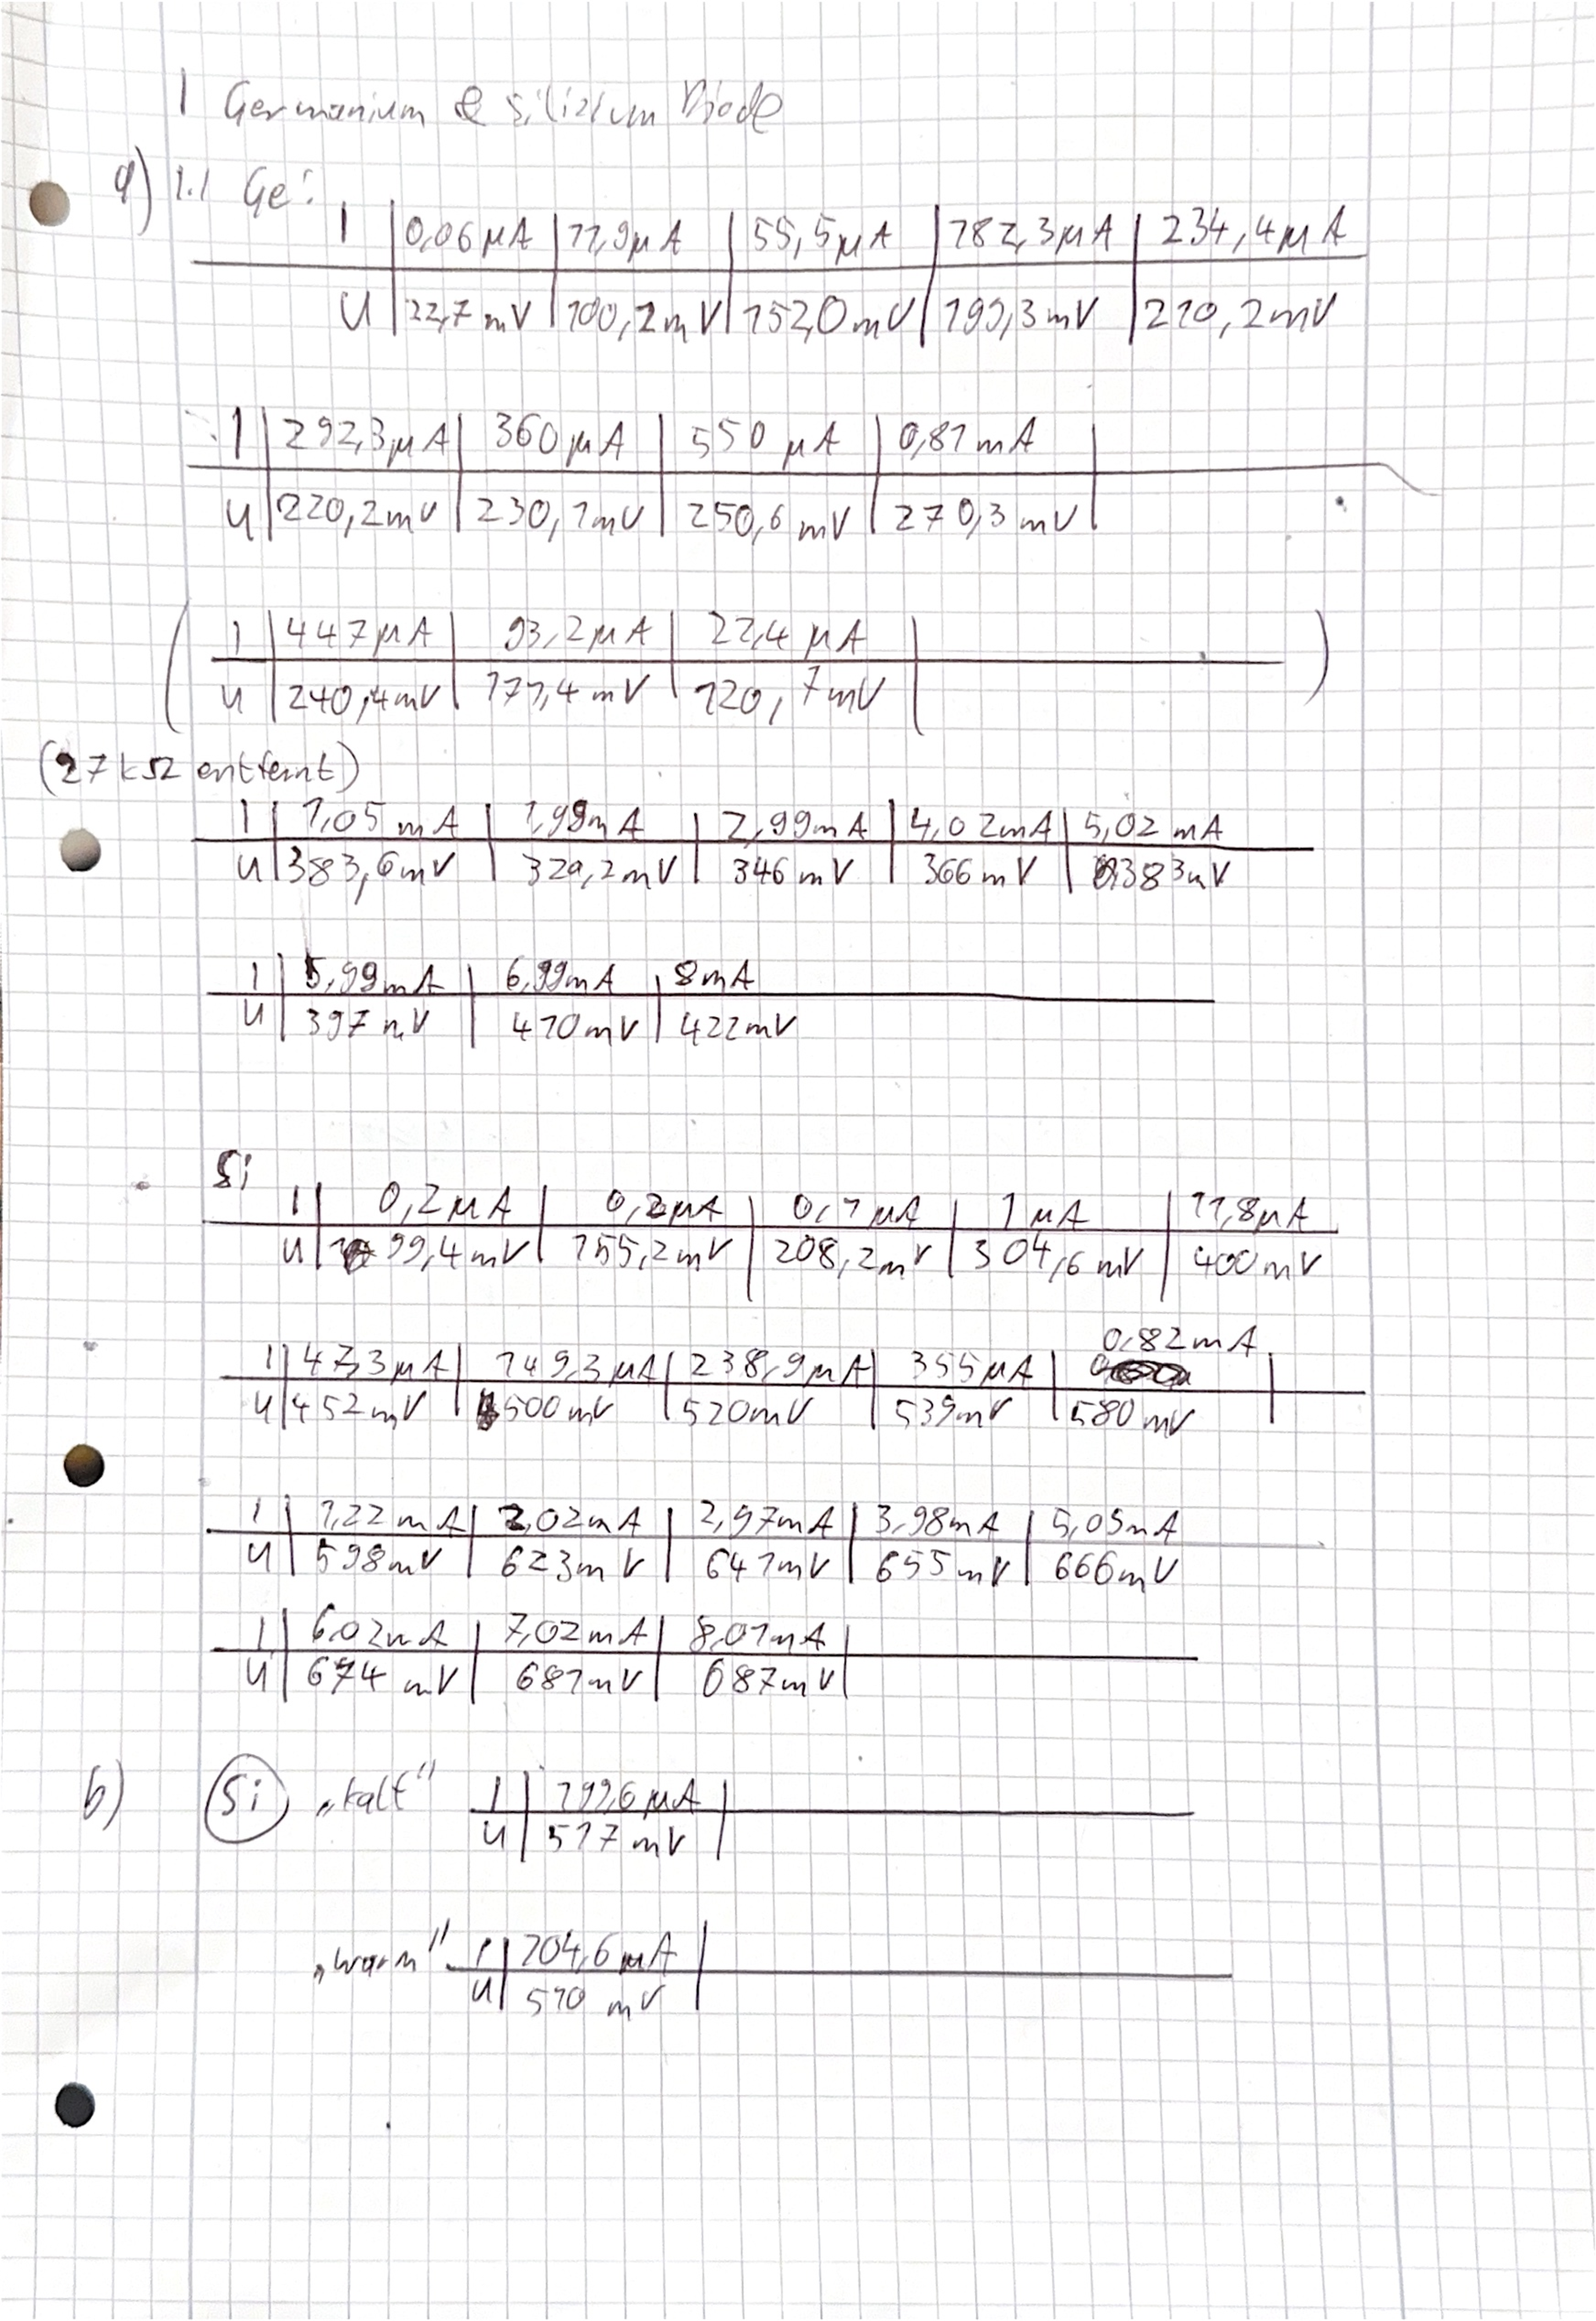
\includepdf[pages=-]{MessprotDioden.pdf}

\end{document}